\subsection{課題説明}
3種類の連続関数$y=x^2$、$z=x^2+y^2$、$y=-x \times \cos(x)$について、
最急降下法の適用を通して探索挙動を観察した。
以下では,最急降下法のアルゴリズムについて
フローチャートを用いて解説する。
その後、3種類の関数毎にプログラムの変更箇所、
観察意図観察方法、観察結果、考察について説明する。


\subsection{Level 2共通部分}

\subsubsection{最急降下法のアルゴリズム}
最急降下法とは
\begin{oframed}
微分値を基にxを移動させる幅を決定する際
\begin{align*}
x_{next} = x - \alpha * f'(x)
\end{align*}
によって移動先を算出するアルゴリズムである.\cite{info2-search1}
\end{oframed}

微分値はその対象のモデル式における切片の傾きに等しい.
つまり,ある点から切片を引き,そこに対して学習係数文移動させる方法である.
最急降下法の名前の通り,関数の最小値へと引き寄せられるように移動していく.
尚最大値を求める場合は,学習係数$\alpha$を符号反転させれば良い.
この際,探索点が移動した場所を可視化すると,より良い精度の場合はモデル式と同じグラフを辿ると考える.

また最急降下法を用いた今回のCプログラムsteepest\_decent.cについてフローチャート図を用いて解説を行う. (図:\ref{fig:flowsttep})

\begin{figure}[H]
\centering
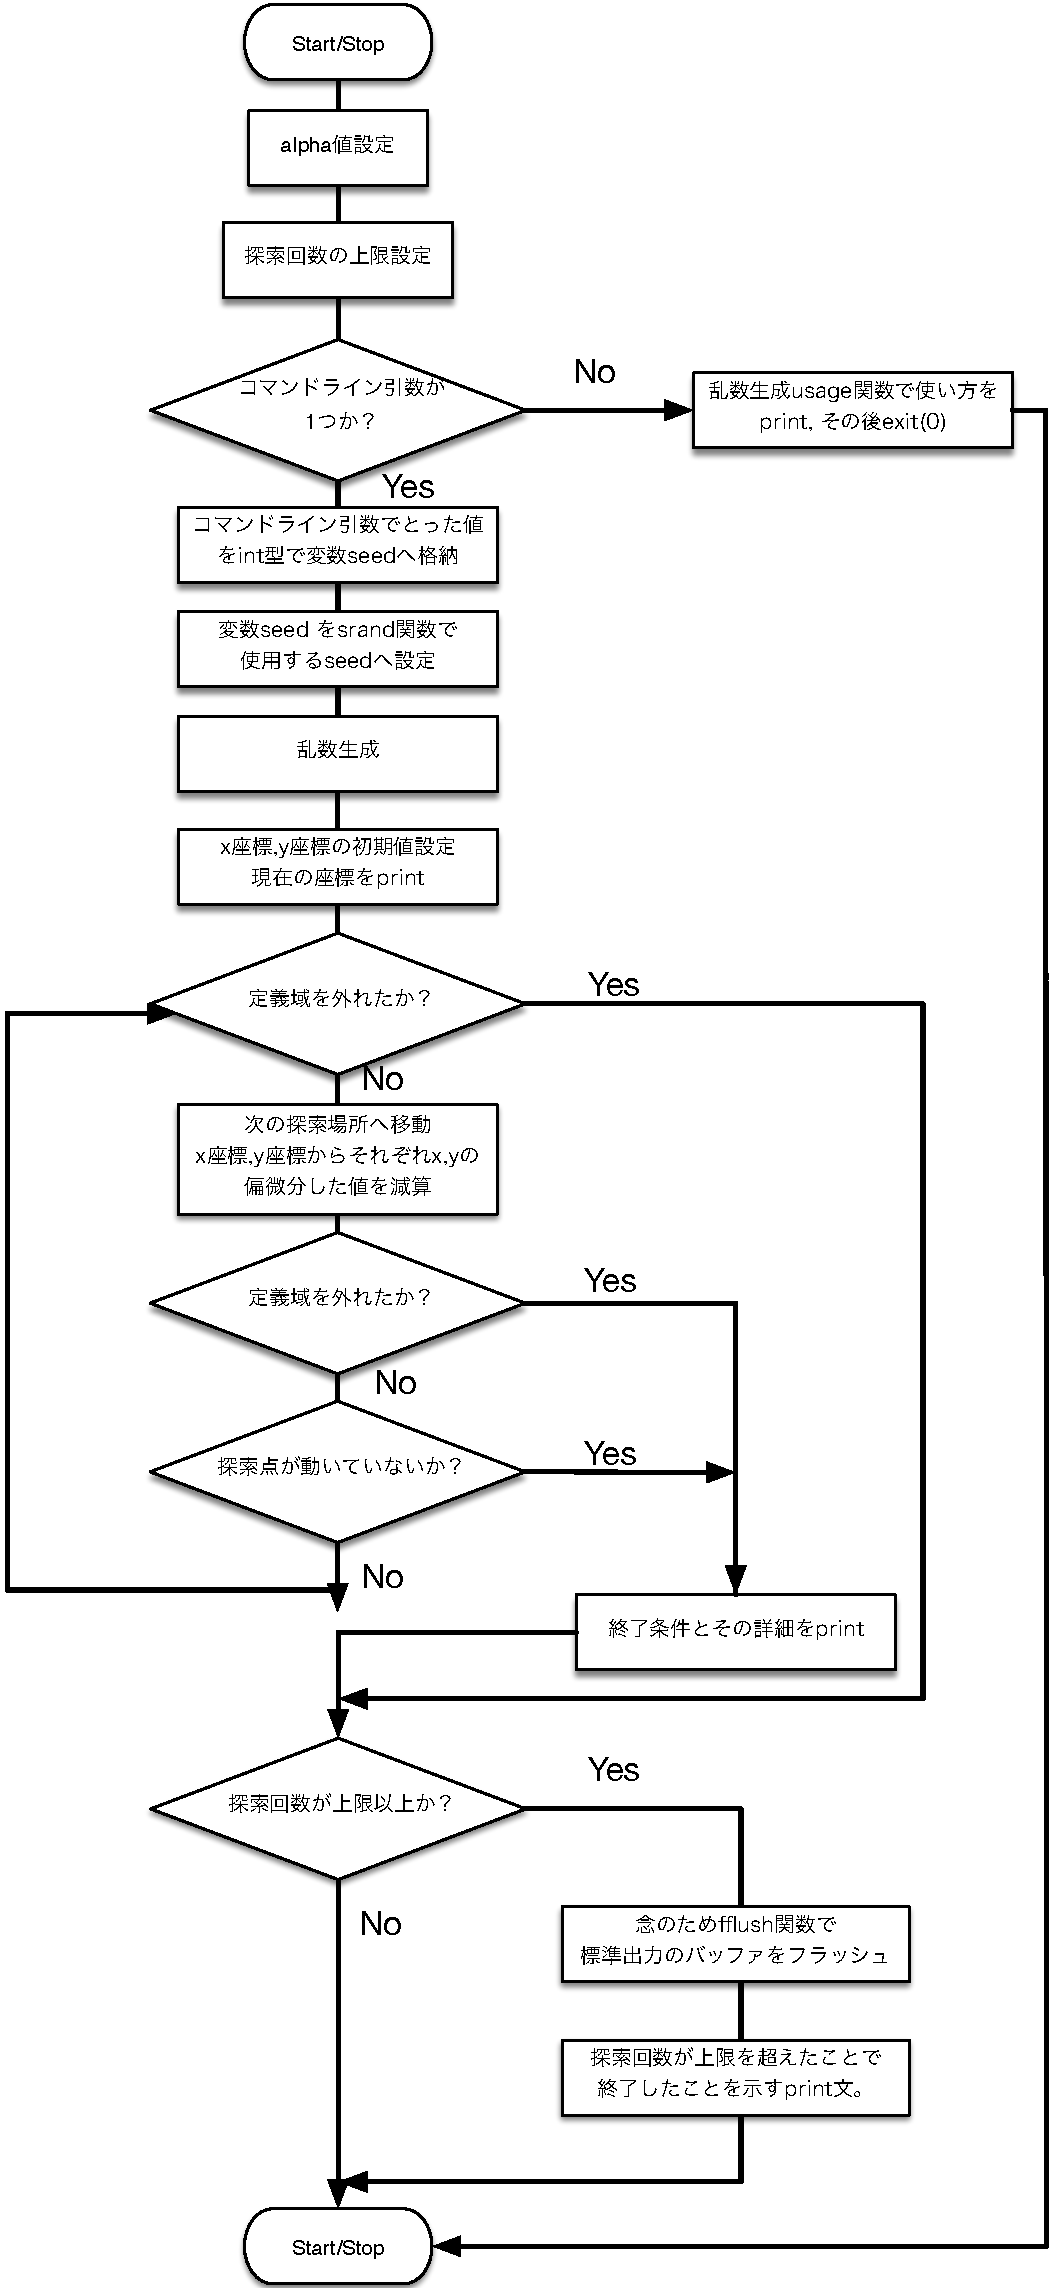
\includegraphics[width=0.5\textwidth]{figs/flowchart.pdf}
\caption{steepest\_decent.cのフローチャート図}
\label{fig:flowsttep}
\end{figure}

このCプログラムは,フローチャート図に示す通り探索場所を移動する度に定義域,mた前回との探索場所の移動について分岐させ,最適解を見つけ出すプログラムである.
最急降下法を用いるにあって,このプログラムではプログラマがソースコード中にモデル式及び偏微分を行った結果を入力する必要がある.
今回の実験ではlevel2の課題はこのCプログラムをそのまま,又は一部変更して利用した.

